\hypertarget{Digital Twin Implementation}{%
\section{Digital Twin Implementation}\label{Digital Twin Implementation}}

Traditionally, automotive industry has long practiced the gradual transition from virtual, to hybrid, to physical phases within an X-in-the-loop (XIL; X = model, software, processor, hardware, vehicle) framework. Furthermore, recent modeling \& simulation methodologies such as simulation-as-a-service (SAAS) complemented with simulation-to-reality (sim2real) transfer show promise in facilitating parallelized scenario-based validation to enable robust system development and comprehensive corner-case analysis. However, the lack of physically realistic simulation of perception characteristics, system dynamics and agent-environment interactions, along with associated uncertainties, restricts the scalability and reliability of simulation-based verification. 

In such a milieu, digital twins have emerged as potentially viable tools to improve simulation fidelity and to develop adaption/augmentation techniques that can help bridge the sim2real gap. The following sections delve into the development of physically and graphically accurate vehicle and environment digital twins, and also discuss the integration of these with APIs and HMIs for developing autonomy-oriented applications.

\hypertarget{Vehicle Digital Twins}{%
\subsection{Vehicle Digital Twins}\label{Vehicle Digital Twins}}

\begin{figure}[t]
    \centering
    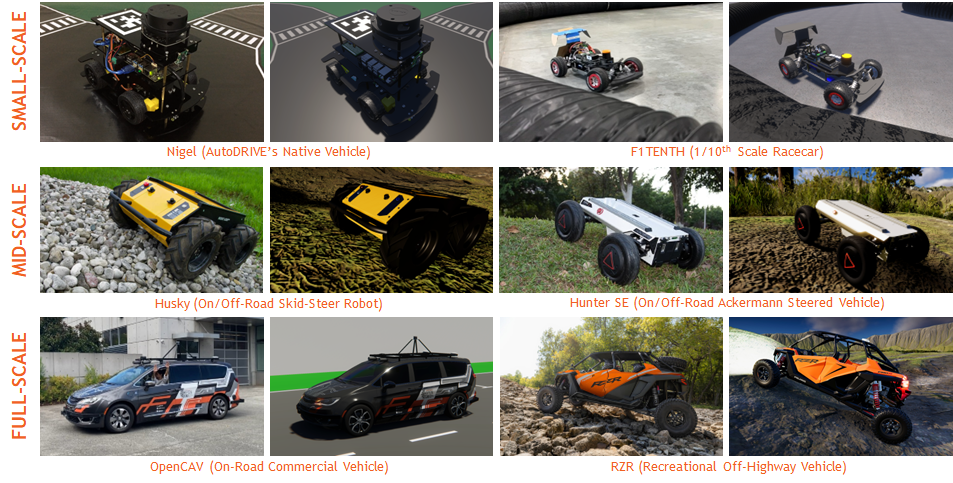
\includegraphics[width=\linewidth]{Figures/fig4.png}
    \caption{Autonomy-oriented vehicle digital twins across scales: Nigel and F1TENTH (small-scale), Husky and Hunter SE (mid-scale), and OpenCAV and RZR (full-scale) platforms for on/off-road autonomy.}
    \label{fig: figure4}
\end{figure}

As described earlier, we leveraged AutoDRIVE Simulator \cite{AutoDRIVESimulator, AutoDRIVESimulatorReport} to develop digital twin models of six different vehicles, across different scales and ODDs (Fig. \ref{fig: figure4}). These included small-scale (Nigel and F1TENTH), mid-scale (Husky and Hunter SE) and full-scale (OpenCAV and RZR) vehicles targeted towards on-road as well as off-road autonomy. It is to be noted that Husky and RZR fall purely under off-road ODD, and since this project (as well as Autoware) primarily targets on-road autonomy, these platforms have not been discussed elaborately in this report. Consequently, the following sections describe the digital twins of Nigel, F1TENTH, Hunter SE and OpenCAV in detail. This elucidation covers details at component, sub-system, system, all the way up to complex system-of-systems level models and their interconnects.

From a computational perspective, the said simulation framework was developed modularly using object-oriented programming (OOP) constructs. Additionally, the simulator took advantage of CPU multi-threading as well as GPU instancing (if available) to efficiently handle the workload, while providing cross-platform support.

\subsubsection{Vehicle Models}
\label{Vehicle Models}

\begin{figure}[t]
    \centering
    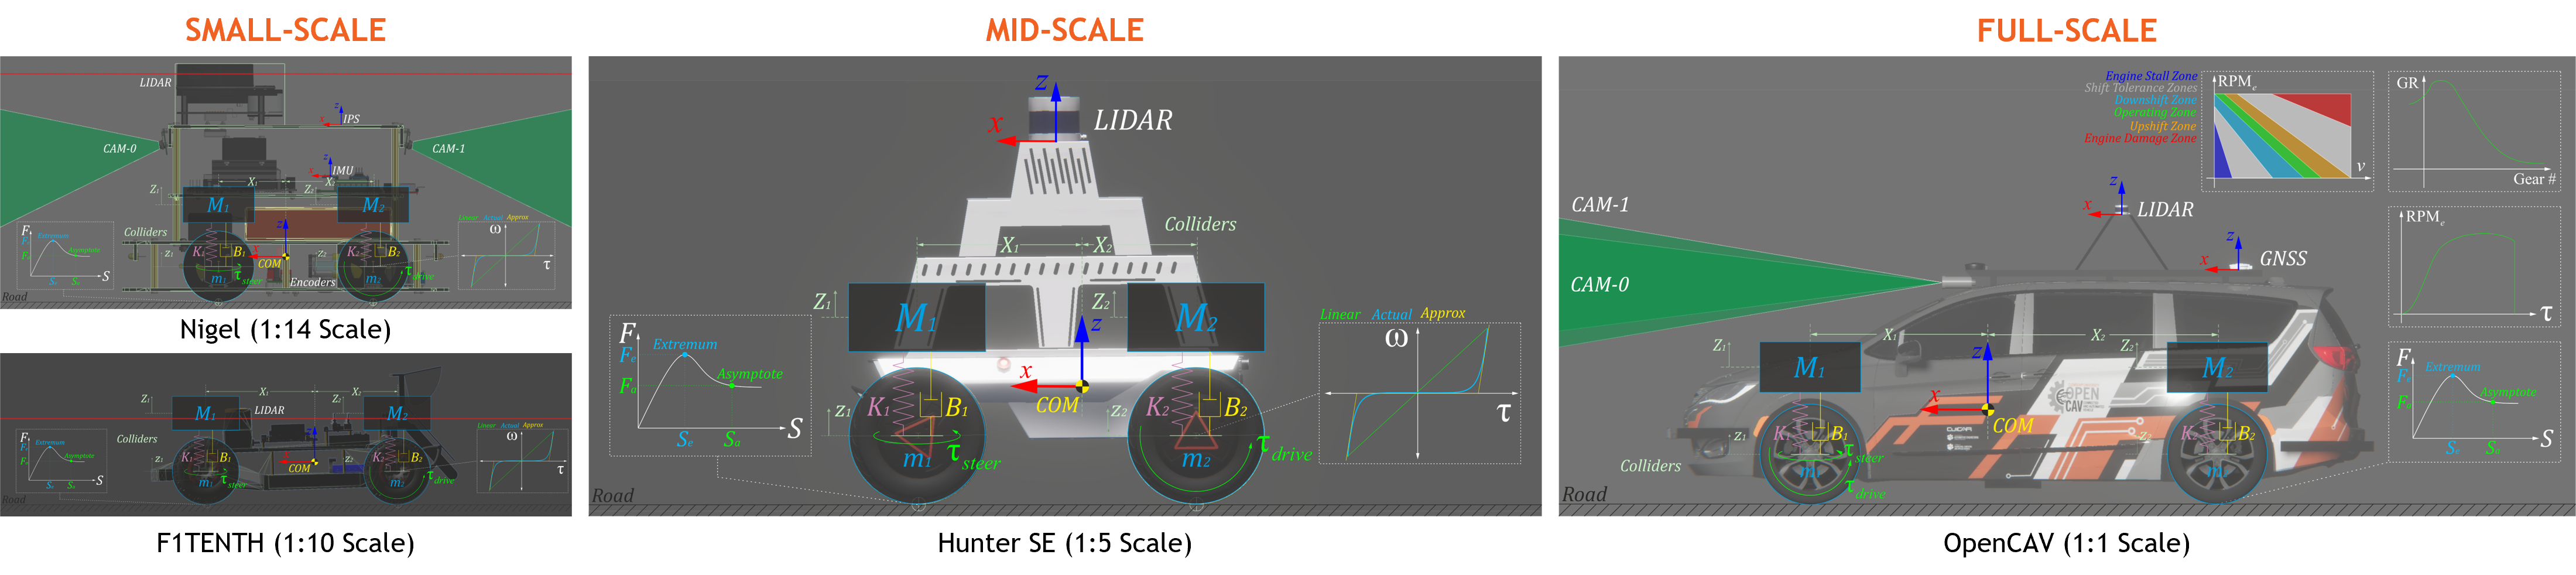
\includegraphics[width=\linewidth]{Figures/fig5.png}
    \caption{Simulation of vehicle dynamics, sensors and actuators for Nigel and F1TENTH digital twins.}
    \label{fig: figure5}
\end{figure}

The vehicles (refer Fig. \ref{fig: figure5}) are conjunctly modeled using sprung-mass ${^iM}$ and rigid-body representations. Here, the total mass $M=\sum{^iM}$, center of mass, $X_{COM} = \frac{\sum{{^iM}*{^iX}}}{\sum{^iM}}$ and moment of inertia $I_{COM} = \sum{{^iM}*{^iX^2}}$, serve as the linkage between these two representations, where ${^iX}$ represents the coordinates of the sprung masses. Each vehicle's wheels are also modeled as rigid bodies with mass $m$, experiencing gravitational and suspension forces: ${^im} * {^i{\ddot{z}}} + {^iB} * ({^i{\dot{z}}}-{^i{\dot{Z}}}) + {^iK} * ({^i{z}}-{^i{Z}})$.

\paragraph{Powertrain Dynamics}
\label{Powertrain Dynamics}

For small and mid-scale vehicles, which usually implement an electric motor for propulsion, the front/rear/all wheels are driven by applying a torque ${^i\tau_{drive}} = {^iI_w}*{^i\dot{\omega}_w}$, where ${^iI_w} = \frac{1}{2}*{^im_w}*{^i{r_w}^2}$ represents the moment of inertia, $^i\dot{\omega}_w$ is the angular acceleration, $^im_w$ is the mass, and $^ir_w$ is the radius of the $i$-th wheel. The actuation delays can also be modeled by splitting the torque profile into multiple segments based on operating conditions. For full-scale vehicles, however, the powertrain comprises an engine, transmission and differential. The engine is modeled based on its torque-speed characteristics. The engine RPM is updated smoothly based on its current value $RPM_e$, the idle speed $RPM_i$, average wheel speed $RPM_w$, final drive ratio $FDR$, current gear ratio $GR$, and the vehicle velocity $v$. The update can be expressed as $RPM_e := \left[RPM_i + \left(|RPM_w| \times FDR * GR\right)\right]_{(RPM_e,v)}$ where, $[\mathscr{F}]_x$ denotes evaluation of $\mathscr{F}$ at $x$. The total torque generated by the powertrain is computed as $\tau_{\text{total}} = \left[\tau_e\right]_{RPM_e} * \left[GR\right]_{G_\#} * FDR * T * \mathscr{A}$. Here, $\tau_e$ is the engine torque, $T$ is the throttle input, and $\mathscr{A}$ is a non-linear smoothing operator which increases the vehicle acceleration based on the throttle input. The automatic transmission decides to upshift/downshift the gears based on the transmission map of a given vehicle. This keeps the engine RPM in a good operating range for a given speed: $RPM_e = \frac{{v_{\text{MPH}} * 5280 * 12}}{{60 * 2 * \pi * R_{\text{tire}}}} * FDR * GR$. It is to be noted that while shifting the gears, the total torque produced by the powertrain is set to zero to simulate the clutch disengagement. It is also noteworthy that the auto-transmission is put in neutral gear once the vehicle is in standstill condition and parking gear if handbrakes are engaged in standstill condition. Additionally, switching between drive and reverse gears requires that the vehicle first be in the neutral gear to allow this transition. The total torque $\tau_\text{total}$ from the drivetrain is divided to the wheels based on the drive configuration of the vehicle:
$
\tau_{\text{out}} = \begin{cases}
\frac{\tau_{\text{total}}}{2} & \text{if FWD/RWD} \\
\frac{\tau_{\text{total}}}{4} & \text{if AWD}
\end{cases}
$
The torque transmitted to wheels $\tau_w$ is modeled by dividing the output torque $\tau_\text{out}$ to the left and right wheels based on the steering input. The left wheel receives a torque amounting to $^{L}\tau_{w} = \tau_{\text{out}} * (1 - \tau_{\text{drop}} * |\delta^{-}|)$, while the right wheel receives a torque equivalent to $^{R}\tau_{w} = \tau_{\text{out}} * (1 - \tau_{\text{drop}} * |\delta^{+}|)$. Here, $\tau_\text{drop}$ is the torque-drop at differential and $\delta^{\pm}$ indicates positive and negative steering angles, respectively. The value of $(\tau_{\text{drop}} * |\delta^{\pm}|)$ is clamped between $[0,0.9]$.

\paragraph{Brake Dynamics}
\label{Brake Dynamics}

The driving actuators for small and mid-scale vehicles simulate braking torque by applying a holding torque in idle conditions, i.e., ${^i\tau_\text{brake}} = {^i\tau_\text{idle}}$. For full-scale vehicles, the braking torque is modeled as ${^i\tau_\text{brake}} = \frac{{^iM}*v^2}{2*D_\text{brake}}*R_b$ where $R_b$ is the brake disk radius and $D_\text{brake}$ is the braking distance at 60 MPH, which can be obtained from physical vehicle tests. This braking torque is applied to the wheels based on the type of brake input: for combi-brakes, this torque is applied to all the wheels, and for handbrakes, it is applied to the rear wheels only.

\paragraph{Steering Dynamics}
\label{Steering Dynamics}

The steering mechanism operates by employing a steering actuator, which applies a torque $\tau_{\text{steer}}$ to achieve the desired steering angle $\delta$ with a smooth rate $\dot{\delta}$, without exceeding the steering limits $\pm \delta_\text{lim}$. The rate at which the vehicle steers is governed by its speed $v$ and steering sensitivity $\kappa_\delta$, and is represented as $\dot{\delta} = \kappa_\delta + \kappa_v * \frac{v}{v_\text{max}}$. Here, $\kappa_v$ is the speed-dependency factor of the steering mechanism. Finally, the individual angle for left $\delta_l$ and right $\delta_r$ wheels are governed by the Ackermann steering geometry, considering the wheelbase $l$ and track width $w$ of the vehicle:
$
\left\{
\begin{matrix} 
\delta_l = \textup{tan}^{-1}\left(\frac{2*l*\textup{tan}(\delta)}{2*l+w*\textup{tan}(\delta)}\right) \\ 
\delta_r = \textup{tan}^{-1}\left(\frac{2*l*\textup{tan}(\delta)}{2*l-w*\textup{tan}(\delta)}\right) 
\end{matrix}
\right.
$.

\paragraph{Suspension Dynamics}
\label{Suspension Dynamics}

For small and mid-scale vehicles, the suspension force acting on each sprung mass is calculated as ${^iM} * {^i{\ddot{Z}}} + {^iB} * ({^i{\dot{Z}}}-{^i{\dot{z}}}) + {^iK} * ({^i{Z}}-{^i{z}})$, where $^iZ$ and $^iz$ denote the displacements of the sprung and unsprung masses, respectively, and $^iB$ and $^iK$ represent the damping and spring coefficients of the $i$-th suspension. For full-scale vehicles, however, the stiffness ${^iK} = {^iM} * {^i\omega_n}^2$ and damping $^iB = 2 * ^i\zeta * \sqrt{{^iK} * {^iM}}$ coefficients of the suspension system are computed based on the sprung mass ${^iM}$, natural frequency ${^i\omega_n}$, and damping ratio ${^i\zeta}$ parameters. The point of suspension force application ${^iZ_F}$ is calculated based on the suspension geometry:
${^iZ_F} = {^iZ_\text{COM}} - {^iZ_w} + {^ir_w} - {^iZ_f}$, where $^iZ_\text{COM}$ denotes the Z-component of vehicle's center of mass, $^iZ_w$ is the Z-component of the relative transformation between each wheel and the vehicle frame ($^VT_{w_i}$), $^ir_w$ is the wheel radius, and $^iZ_f$ is the force offset determined by the suspension geometry. Lastly, the suspension displacement $^iZ_s$ at any given moment can be computed as ${^iZ_s} = \frac{{^iM} * g}{{^iZ_0} * {^iK}}$, where $g$ represents the acceleration due to gravity, and $^iZ_0$ is the suspension's equilibrium point. Additionally, full-scale vehicle models also have a provision to include anti-roll bars, which apply a force on the left ${^LF_r} = K_r * {^RZ} - {^LZ}$ and right ${R^F_r} = K_r * {^LZ} - {^RZ}$ wheels as long as they are grounded at the contact point $Z_c$. This force is directly proportional to the stiffness of the anti-roll bar, $K_r$. The left and right wheel travels are given by ${^LZ} = \frac{-{^LZ_c} - {^Lr_w}}{^LZ_s}$ and ${^RZ} = \frac{-{^RZ_c} - {^Rr_w}}{^RZ_s}$.

\paragraph{Tire Dynamics}
\label{Tire Dynamics}

Tire forces are determined based on the friction curve for each tire $\left\{\begin{matrix} {^iF_{t_x}} = F(^iS_x) \\{^iF_{t_y}} = F(^iS_y) \\ \end{matrix}\right.$, where $^iS_x$ and $^iS_y$ represent the longitudinal and lateral slips of the $i$-th tire, respectively. The friction curve is approximated using a two-piece spline, defined as $F(S) = \left\{\begin{matrix} f_0(S); \;\; S_0 \leq S < S_e \\ f_1(S); \;\; S_e \leq S < S_a \\ \end{matrix}\right.$, with $f_k(S) = a_k*S^3+b_k*S^2+c_k*S+d_k$ as a cubic polynomial function. The first segment of the spline ranges from zero $(S_0,F_0)$ to an extremum point $(S_e,F_e)$, while the second segment ranges from the extremum point $(S_e, F_e)$ to an asymptote point $(S_a, F_a)$. Tire slip is influenced by factors including tire stiffness $^iC_\alpha$, steering angle $\delta$, wheel speeds $^i\omega$, suspension forces $^iF_s$, and rigid-body momentum ${^iP}={^iM}*{^iv}$. The longitudinal slip $^iS_x$ of $i$-th tire is calculated by comparing the longitudinal components of its surface velocity $v_x$ (i.e., the longitudinal linear velocity of the vehicle) with its angular velocity $^i\omega$: ${^iS_x} = \frac{{^ir}*{^i\omega}-v_x}{v_x}$. The lateral slip $^iS_y$ depends on the tire's slip angle $\alpha$ and is determined by comparing the longitudinal $v_x$ (forward velocity) and lateral $v_y$ (side-slip velocity) components of the vehicle's linear velocity: ${^iS_y} = \tan(\alpha) = \frac{v_y}{\left| v_x \right|}$.

\paragraph{Aerodynamics}
\label{Aerodynamics}

Small and mid-scale vehicles are modeled with constant coefficients for linear $F_d$ as well as angular $T_d$ drags, which act directly proportional to their linear $v$ and angular $\omega$ velocities. These vehicles do not create significant downforce due to unoptimized aerodynamics, limited velocities and smaller size and mass. Full-scale vehicles, on the other hand, have been modeled to simulate variable air drag $F_\text{aero}$ acting on the vehicle, which is computed based on the vehicle’s operating condition:
$
F_{\text{aero}} = \begin{cases}
F_{d_\text{max}} & \text{if } v \geq v_{\text{max}} \\
F_{d_\text{idle}} & \text{if } \tau_{\text{out}} = 0 \\
F_{d_\text{rev}} & \text{if } (v \geq v_{\text{rev}}) \land (G_\# = -1) \land (RPM_{w} < 0) \\
F_{d_\text{idle}} & \text{otherwise}
\end{cases}
$
where, $v$ is the vehicle velocity, $v_\text{max}$ is the vehicle's designated top-speed, $v_\text{rev}$ is the vehicle's designated maximum reverse velocity, $G_\#$ is the operating gear, and $RPM_w$ is the average wheel RPM. The downforce acting on a full-scale vehicle is modeled proportional to its velocity: $F_\text{down}=K_\text{down}*|v|$, where $K_\text{down}$ is the downforce coefficient.

\subsubsection{Sensor Models}
\label{Sensor Models}

The simulated vehicles can be equipped with physically accurate interoceptive and exteroceptive sensing modalities.

\paragraph{Actuator Feedbacks}
\label{Actuator Feedbacks}

Throttle ($\tau$) and steering ($\delta$) sensors are simulated using a simple feedback loop.

\paragraph{Incremental Encoders}
\label{Incremental Encoders}

Simulated incremental encoders measure wheel rotations $^iN_{\text{ticks}} = {^iPPR} \times {^iCGR} \times {^iN_{\text{rev}}}$, where $^iN_{\text{ticks}}$ represents the measured ticks, $^iPPR$ is the encoder resolution (pulses per revolution), $^iCGR$ is the cumulative gear ratio, and $^iN_{\text{rev}}$ represents the wheel revolutions.

\paragraph{Inertial Navigation Systems}
\label{Inertial Navigation Systems}

Positioning systems and inertial measurement units (IMU) are simulated based on temporally coherent rigid-body transform updates of the vehicle $\{v\}$ with respect to the world $\{w\}$: ${^w\mathbf{T}_v} = \left[\begin{array}{c | c} \mathbf{R}_{3 \times 3} & \mathbf{t}_{3 \times 1} \\ \hline \mathbf{0}_{1 \times 3} & 1 \end{array}\right] \in SE(3)$. The positioning systems provide 3-DOF positional coordinates $\{x,y,z\}$ of the vehicle, while the IMU supplies linear accelerations $\{a_x,a_y,a_z\}$, angular velocities $\{\omega_x,\omega_y,\omega_z\}$, and 3-DOF orientation data for the vehicle, either as Euler angles $\{\phi_x,\theta_y,\psi_z\}$ or as a quaternion $\{q_0,q_1,q_2,q_3\}$.

\paragraph{Planar LIDARs}
\label{Planar LIDARs}

2D LIDAR simulation employs iterative ray-casting \texttt{raycast}\{$^w\mathbf{T}_l$, $\vec{\mathbf{R}}$, $r_{\text{max}}$\} for each angle $\theta \in \left [ \theta_{\text{min}}:\theta_{\text{res}}:\theta_{\text{max}} \right ]$ at a specified update rate. Here, ${^w\mathbf{T}_l} = {^w\mathbf{T}_v} * {^v\mathbf{T}_l} \in SE(3)$ represents the relative transformation of the LIDAR \{$l$\} with respect to the vehicle \{$v$\} and the world \{$w$\}, $\vec{\mathbf{R}} = \left [\cos(\theta) \;\; \sin(\theta) \;\; 0 \right ]^T$ defines the direction vector of each ray-cast $R$, where $r_{\text{min}}$ and $r_{\text{max}}$ denote the minimum and maximum linear ranges, $\theta_{\text{min}}$ and $\theta_{\text{max}}$ denote the minimum and maximum angular ranges, and $\theta_{\text{res}}$ represents the angular resolution of the LIDAR, respectively. The laser scan ranges are determined by checking ray-cast hits and then applying a threshold to the minimum linear range of the LIDAR, calculated as \texttt{ranges[i]}$=\begin{cases} \texttt{hit.dist} & \text{ if } \texttt{ray[i].hit} \text{ and } \texttt{hit.dist} \geq r_{\text{min}} \\ \infty & \text{ otherwise} \end{cases}$, where \texttt{ray.hit} is a Boolean flag indicating whether a ray-cast hits any colliders in the scene, and \texttt{hit.dist}$=\sqrt{(x_{\text{hit}}-x_{\text{ray}})^2 + (y_{\text{hit}}-y_{\text{ray}})^2 + (z_{\text{hit}}-z_{\text{ray}})^2}$ calculates the Euclidean distance from the ray-cast source $\{x_{\text{ray}}, y_{\text{ray}}, z_{\text{ray}}\}$ to the hit point $\{x_{\text{hit}}, y_{\text{hit}}, z_{\text{hit}}\}$.

\paragraph{Spatial LIDARs}
\label{Spatial LIDARs}

3D LIDAR simulation adopts multi-channel parallel ray-casting \texttt{raycast}\{$^w\mathbf{T}_l$, $\vec{\mathbf{R}}$, $r_{\text{max}}$\} for each angle $\theta \in \left [ \theta_{\text{min}}:\theta_{\text{res}}:\theta_{\text{max}} \right ]$ and each channel $\phi \in \left [ \phi_{\text{min}}:\phi_{\text{res}}:\phi_{\text{max}} \right ]$ at a specified update rate, with GPU acceleration (if available). Here, ${^w\mathbf{T}_l} = {^w\mathbf{T}_v} * {^v\mathbf{T}_l} \in SE(3)$ represents the relative transformation of the LIDAR \{$l$\} with respect to the vehicle \{$v$\} and the world \{$w$\}, $\vec{\mathbf{R}} = \left [\cos(\theta)*\cos(\phi) \;\; \sin(\theta)*\cos(\phi) \;\; -\sin(\phi) \right ]^T$ defines the direction vector of each ray-cast $R$, where $r_{\text{min}}$ and $r_{\text{max}}$ denote the minimum and maximum linear ranges, $\theta_{\text{min}}$ and $\theta_{\text{max}}$ denote the minimum and maximum horizontal angular ranges, $\phi_{\text{min}}$ and $\phi_{\text{max}}$ denote the minimum and maximum vertical angular ranges, and $\theta_{\text{res}}$ and $\phi_{\text{res}}$ represent the horizontal and vertical angular resolutions of the LIDAR, respectively. The thresholded ray-cast hit coordinates $\{x_{\text{hit}}, y_{\text{hit}}, z_{\text{hit}}\}$, from each of the casted rays is encoded into byte arrays based on the LIDAR parameters, and given out as the point cloud data.

\paragraph{Cameras}
\label{Cameras}

Simulated cameras are parameterized by their focal length $f=$, sensor size $\{s_x, s_y\}$, target resolution, as well as the distances to the near $N$ and far $F$ clipping planes. The viewport rendering pipeline for the simulated cameras operates in three stages. First, the camera view matrix $\mathbf{V} \in SE(3)$ is computed by obtaining the relative homogeneous transform of the camera $\{c\}$ with respect to the world $\{w\}$: $\mathbf{V} = \begin{bmatrix} r_{00} & r_{01} & r_{02} & t_{0} \\ r_{10} & r_{11} & r_{12} & t_{1} \\ r_{20} & r_{21} & r_{22} & t_{2} \\ 0 & 0 & 0 & 1 \\ \end{bmatrix}$, where $r_{ij}$ and $t_i$ denote the rotational and translational components, respectively. Next, the camera projection matrix $\mathbf{P} \in \mathbb{R}^{4 \times 4}$ is calculated to project world coordinates into image space coordinates: $\mathbf{P} = \begin{bmatrix} \frac{2*N}{R-L} & 0 & \frac{R+L}{R-L} & 0 \\ 0 & \frac{2*N}{T-B} & \frac{T+B}{T-B} & 0 \\ 0 & 0 & -\frac{F+N}{F-N} & -\frac{2*F*N}{F-N} \\ 0 & 0 & -1 & 0 \\ \end{bmatrix}$, where $L$, $R$, $T$, and $B$ denote the left, right, top, and bottom offsets of the sensor. The camera parameters $\{f,s_x,s_y\}$ are related to the terms of the projection matrix as follows: $f = \frac{2*N}{R-L}$, $a = \frac{s_y}{s_x}$, and $\frac{f}{a} = \frac{2*N}{T-B}$. The perspective projection from the simulated camera's viewport is given as $\mathbf{C} = \mathbf{P}*\mathbf{V}*\mathbf{W}$, where $\mathbf{C} = \left [x_c\;\;y_c\;\;z_c\;\;w_c \right ]^T$ represents image space coordinates, and $\mathbf{W} = \left [x_w\;\;y_w\;\;z_w\;\;w_w \right ]^T$ represents world coordinates. Finally, this camera projection is transformed into normalized device coordinates (NDC) by performing perspective division (i.e., dividing throughout by $w_c$), leading to a viewport projection achieved by scaling and shifting the result and then utilizing the rasterization process of the graphics API (e.g., DirectX for Windows, Metal for macOS, and Vulkan for Linux). Additionally, a post-processing step simulates non-linear lens and film effects, such as lens distortion, depth of field, exposure, ambient occlusion, contact shadows, bloom, motion blur, film grain, chromatic aberration, etc.

\subsubsection{Calibration and Validation}
\label{Sub-Section: Calibration and Validation}

The vehicle digital twin models were calibrated and validated against geometric, static and dynamic measurement data collected from their real-world counterparts and/or their datasheets. This included the validation of geometric measurements for physical as well as visual purposes, static calibration for mass and center of mass parameters and dynamic calibration for validating standard benchmark maneuvers performed in open-loop tests. Additionally, sensor models were validated against static and dynamic characteristics of their real-world counterparts. Fig. \ref{fig: figure6} depicts some of these calibration/validation tests.

\begin{figure}[t]
    \centering
    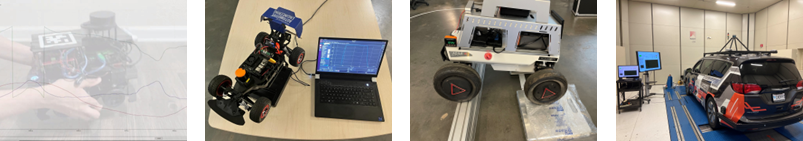
\includegraphics[width=\linewidth]{Figures/fig6.png}
    \caption{Calibration and validation of vehicle digital twins: IMU calibration/validation of Nigel, VESC calibration/validation of F1TENTH, static measurements of Hunter SE, and powertrain measurements of OpenCAV.}
    \label{fig: figure6}
\end{figure}

\subsubsection{Physical Vehicle Build and Setup}
\label{Sub-Section: Physical Vehicle Build and Setup}

We predominantly worked with two small-scale physical vehicles during the course of this project. These included an F1TENTH and a Nigel. While the prior was acquired off-the-shelf, its hardware and software had to be tested, configured, calibrated and set up to interface with the \href{https://github.com/Tinker-Twins/AutoDRIVE-F1TENTH}{ROS}, \href{https://github.com/Tinker-Twins/AutoDRIVE-F1TENTH}{ROS 2} and \href{https://github.com/Tinker-Twins/AutoDRIVE-Autoware}{Autoware} stacks. The latter, on the other hand, was designed, manufactured and assembled from scratch, including its \href{https://github.com/AutoDRIVE-Ecosystem/Nigel-SolidWorks}{mechanical} and \href{https://github.com/AutoDRIVE-Ecosystem/Nigel-Fritzing}{electronic} subsystems, \href{https://github.com/AutoDRIVE-Ecosystem/Nigel-Arduino}{firmware development} as well as \href{https://github.com/Tinker-Twins/AutoDRIVE/tree/AutoDRIVE-Devkit/ADSS Toolkit/autodrive_ros/autodrive_nigel}{ROS}, \href{https://github.com/Tinker-Twins/AutoDRIVE/tree/AutoDRIVE-Devkit/ADSS Toolkit/autodrive_ros2/autodrive_nigel}{ROS 2} and \href{https://github.com/Tinker-Twins/AutoDRIVE-Autoware}{Autoware} integration.

\begin{figure}[h]
    \centering
    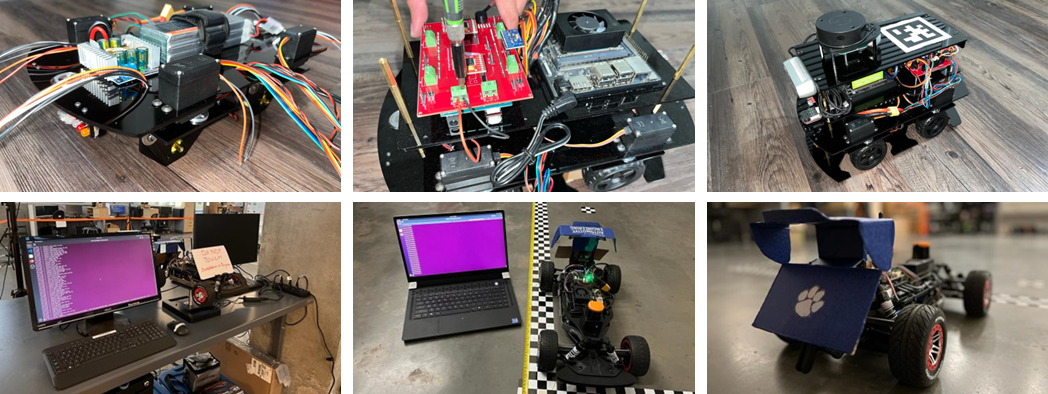
\includegraphics[width=\linewidth]{Figures/fig7.png}
    \caption{Physical build and setup depicting the progress stages during the hardware/software build, calibration and testing of F1TENTH and Nigel vehicles.}
    \label{fig: figure7}
\end{figure}

Being open-source vehicles, build documentation for \href{https://f1tenth.org/build.html}{F1TENTH} and \href{https://github.com/Tinker-Twins/AutoDRIVE/blob/AutoDRIVE-Testbed/Documents/Nigel - Assembly Guide.pdf}{Nigel} are readily available online. Fig. \ref{fig: figure7} depicts intermittent stages in building and setting up these vehicles.

\hypertarget{Environment Digital Twins}{%
\subsection{Environment Digital Twins}\label{Environment Digital Twins}}

\begin{figure}[h]
    \centering
    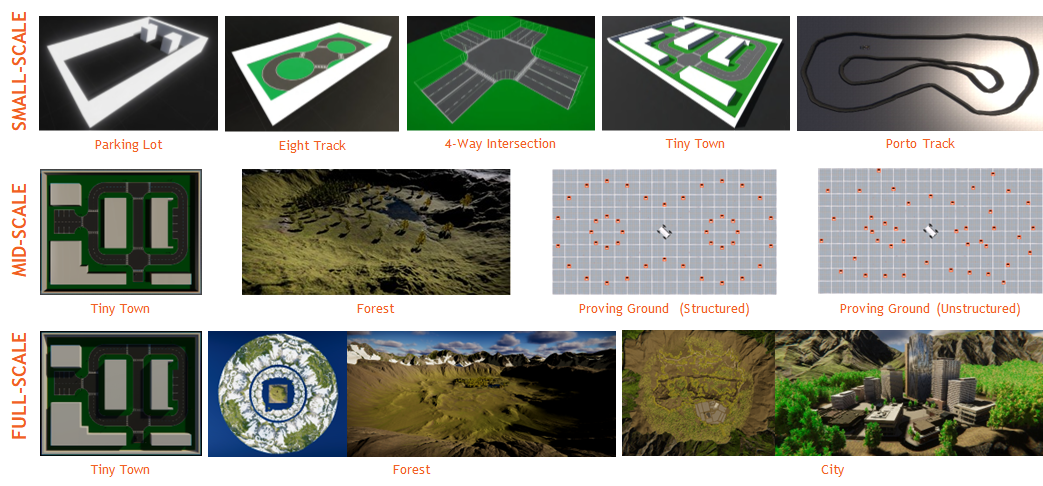
\includegraphics[width=\linewidth]{Figures/fig8.png}
    \caption{Autonomy-oriented environment digital twins across scales: Parking Lot, Eight Track, 4-Way Intersection, Tiny Town and Porto Track (small-scale), Tiny Town, Forest and Proving Ground (mid-scale), and Tiny Town, Forest and City (full-scale) scenarios for on/off-road autonomy.}
    \label{fig: figure8}
\end{figure}

As described earlier, we leveraged AutoDRIVE Simulator \cite{AutoDRIVESimulator, AutoDRIVESimulatorReport} to develop digital twin models of various environments, across different scales and ODDs (Fig. \ref{fig: figure8}). These included realistic counterparts of small-scale environments such as the Parking Lot, Eight Track, 4-Way Intersection and Tiny Town for Nigel, which were developed using AutoDRIVE IDK, as well as the Porto Track for F1TENTH, which was created based on the binary occupancy grid map of its real-world counterpart. Additionally, simplistic mid-scale and full-scale environments such as the scaled-up versions of Tiny Town along with structured and unstructured Proving Ground scenarios were developed. Finally, two highly detailed, albeit imaginary, mid-scale and full-scale scenarios were developed to support on-road as well as off-road autonomy. These included a City scenario and a Forest environment (Fig. \ref{figure9}). The full-scale variants of these scenarios have several rich features and are large enough to support driving for several minutes, if not a few hours. Additionally, these scenarios allowed the simulation of various environmental conditions, such as different times of day as well as weather conditions, to introduce additional degrees of variability. Finally, environmental physics was simulated accurately by conducting mesh-mesh interference detection and computing contact forces, frictional forces, momentum transfer, as well as linear and angular drag acting on all rigid bodies, at each time step.

\begin{figure}[h]
     \centering
     \begin{subfigure}[b]{0.49\linewidth}
         \centering
         \includegraphics[width=\linewidth]{Fig9a.png}
         \caption{City}
         \label{fig9a}
     \end{subfigure}
     \hfill
     \begin{subfigure}[b]{0.49\linewidth}
         \centering
         \includegraphics[width=\linewidth]{Fig9b.png}
         \caption{Forest}
         \label{fig9b}
     \end{subfigure}
     \caption{City and Forest environment digital twins depicting their respective highlights and features to support on-road as well as off-road autonomy.}
    \label{figure9}
\end{figure}

From a computational perspective, the said environment digital twins, especially the full-scale scenarios, made use of pre-baked lightmaps, which provided the benefits of physics-based lighting while reducing the computational overhead of real-time raytracing. Additionally, the simulator implemented level-of-detail (LOD) culling to gradually degrade the LOD of environmental objects as they moved further away from the scene cameras. However, it was ensured that LOD culling did not affect any of the AV camera sensor(s).

AutoDRIVE Simulator supports various approaches to developing realistic/imaginary environment digital twins:
\begin{itemize}
     \item \textit{AutoDRIVE IDK:} Custom scenarios and maps can be crafted by utilizing the modular and adaptable Infrastructure Development Kit (IDK). This kit provides the flexibility to configure terrain modules, road networks, obstruction modules, and traffic elements. Specifically, the Parking Lot, Eight Track, 4-Way Intersection, Tiny Town and Proving Ground scenarios were developed using AutoDRIVE IDK.

     \item \textit{Plug-In Scenarios:} AutoDRIVE Simulator supports third-party tools, such as RoadRunner \cite{RoadRunner}, and open standards like OpenSCENARIO \cite{OpenSCENARIO} and OpenDRIVE \cite{OpenDRIVE}). This allows users to incorporate a diverse range of plugins, packages, and assets in several standard formats for creating or customizing driving scenarios. Particularly, the autonomous racing scenario was created based on the binary occupancy grid map of a real-world F1TENTH racetrack called ``Porto'' using a third-party 3D modeling software, which was then imported into AutoDRIVE Simulator and post-processed with physical as well as graphical enhancements to make it ``sim-ready''.

     \item \textit{Unity Terrain Integration:} Since the AutoDRIVE Simulator is built atop the Unity \cite{Unity} game engine, it seamlessly supports scenario design and development through Unity Terrain \cite{UnityTerrain}. Users have the option to define terrain meshes, textures, heightmaps, vegetation, skyboxes, wind effects, and more, allowing the design of both on-road and off-road scenarios. This option is well-suited for modeling full-scale environments. Specifically, Forest and City scenes were developed using this technique.
\end{itemize}

\hypertarget{APIs and HMIs to Connect with Digital Twins}{%
\subsection{APIs and HMIs to Connect with Digital Twins}\label{APIs and HMIs to Connect with Digital Twins}}

\begin{figure}[h]
    \centering
    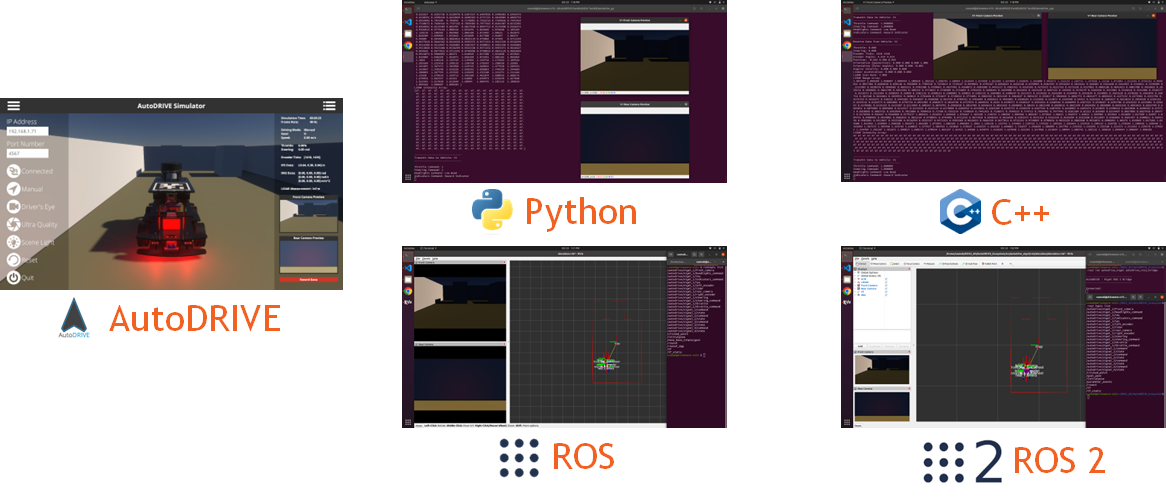
\includegraphics[width=\linewidth]{Figures/fig10.png}
    \caption{APIs to connect with AutoDRIVE Ecosystem: Python, C++, ROS and ROS 2. Note that AutoDRIVE-Autoware integration is accomplished by extending the ROS 2 API.}
    \label{fig: figure10}
\end{figure}

The integration of APIs within the AutoDRIVE Ecosystem was achieved through the comprehensive expansion and incorporation of AutoDRIVE Devkit. The versatile APIs developed as part of this framework facilitate interactions with the virtual/real vehicles using Python, C++, ROS, ROS 2, or the Autoware stack (Fig. \ref{fig: figure10}). This expansion caters to a diverse range of programming preferences, empowering users to exploit the AutoDRIVE Simulator or AutoDRIVE Testbed for swift and flexible development of autonomy algorithms. The framework extends its utility by enabling the development of API-mediated HMIs, catering to both virtual and physical vehicles.

\begin{figure}[t]
    \centering
    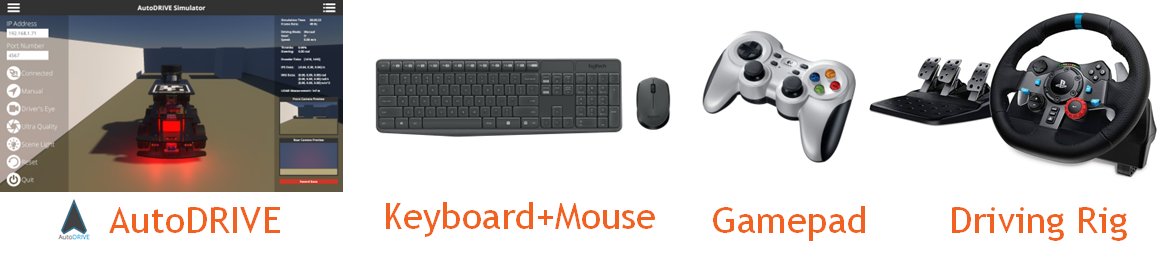
\includegraphics[width=\linewidth]{Figures/fig11.png}
    \caption{HMIs to connect with AutoDRIVE Ecosystem include standard keyboard (digital) and mouse (analog), gamepad/joystick (analog) as well as driving and steering rigs (hybrid).}
    \label{fig: figure11}
\end{figure}

Apart from the API-mediated HMIs, the simulation framework itself served a dual purpose by not only providing a digital twinning platform, but also enabling the development of direct HMIs to interface with the virtual vehicles (Fig. \ref{fig: figure11}). This direct-HMI teleoperation framework, designed for scalability, ensures practical feasibility by relaying identical machine-to-machine (M2M) commands to both virtual and real vehicles. The versatility of this approach allows for a true digital-twin framework, establishing a seamless connection between the simulated environment and the physical world. Additionally, in an extended-reality (XR) setup, this framework offers opportunities to extend the direct-HMI teleoperation to real vehicles, enhancing the applicability and potential of AutoDRIVE Ecosystem in diverse operational scenarios.